\newcommand{\nonterm}[1]{$\langle #1 \rangle$}
\newcommand{\term}[1]{\texttt{#1}}
\newcommand{\RA}{$\Rightarrow$}
\newcommand{\newrule}[1]{\item \nonterm{#1} \RA}
\newcommand{\expr}{\term{EXPRESSION}}


\section{Grammar}
\subsection{LL-Grammar} \label{ll-grammar}

\begin{enumerate}
    \newrule{program} \nonterm{statement} \nonterm{program}
    \newrule{program} \term{func ID(} \nonterm{param-list} \nonterm{func-return-type} \term{\{} \nonterm{func-body} \nonterm{program}
    \newrule{program} \term{EOF}
    \newrule{statement} \nonterm{mutb} \nonterm{define}
    \newrule{statement} \term{ID} \nonterm{id-type}
    \newrule{statement} \term{while} \expr \term{ \{} \nonterm{block-body}
    \newrule{statement} \term{if} \nonterm{cond-clause} \term{\{} \nonterm{block-body} \term{else \{} \nonterm{block-body}
    \newrule{define} \term{ID} \nonterm{define-cont}
    \newrule{define-cont} \term{:} \nonterm{type} \nonterm{opt-assign}
    \newrule{define-cont} \term{=} \nonterm{assign-exp}
    \newrule{opt-assign} \term{=} \nonterm{assign-exp}
    \newrule{opt-assign} \term{$\varepsilon$}
    \newrule{id-type} \term{=} \nonterm{assign-exp}
    \newrule{id-type} \term{(} \nonterm{arg-list}
    \newrule{cond-clause} \term{let ID}
    \newrule{cond-clause} \expr
    \newrule{arg-list} \nonterm{arg} \nonterm{arg-next}
    \newrule{arg-list} \term{)}
    \newrule{arg-next} \term{,} \nonterm{arg} \nonterm{arg-next}
    \newrule{arg-next} \term{)}
    \newrule{arg} \term{ID} \nonterm{opt-arg}
    \newrule{arg} \nonterm{literal}
    \newrule{param-list} \nonterm{param} \nonterm{param-next}
    \newrule{param-list} \term{)}
    \newrule{param-next} \term{,} \nonterm{param} \nonterm{param-next}
    \newrule{param-next} \term{)}
    \newrule{param} \term{LabelID ParamID : } \nonterm{type}
    \newrule{param} \term{\_ ParamID : } \nonterm{type} 
    \newrule{block-body} \nonterm{statement} \nonterm{block-body}
    \newrule{block-body} \term{\}}
    \newrule{func-body} \nonterm{func-statement} \nonterm{func-body}
    \newrule{func-body} \term{\}}
    \newrule{func-statement} \nonterm{mutb} \nonterm{define}
    \newrule{func-statement} \term{ID} \nonterm{id-type}
    \newrule{func-statement} \term{while EXPRESSION \{} \nonterm{func-body}
    \newrule{func-statement} \term{if} \nonterm{cond-clause} \term{\{} \nonterm{func-body}
    \newrule{func-statement} \term{return} \nonterm{opt-ret}
    \newrule{func-return-type} \term{->} \nonterm{type}
    \newrule{func-return-type} \term{$\varepsilon$}
    \newrule{opt-ret} \expr
    \newrule{opt-ret} $\varepsilon$
    \newrule{opt-arg} \term{:} \nonterm{term}
    \newrule{opt-arg} \term{$\varepsilon$}
    \newrule{mutb} \term{var}
    \newrule{mutb} \term{let}
    \newrule{assign-exp} \expr
    \newrule{assign-exp} \nonterm{func-call}
    \newrule{func-call} \term{ID(} \nonterm{arg-list}
    \newrule{type} \term{Int}
    \newrule{type} \term{Double}
    \newrule{type} \term{String}
    \newrule{term} \term{ID}
    \newrule{term} \nonterm{literal}
    \newrule{literal} \term{INT\_LITERAL}
    \newrule{literal} \term{DOUBLE\_LITERAL}
    \newrule{literal} \term{STRING\_LITERAL}
    \newrule{literal} \term{nil}
    

\end{enumerate}
\newpage
\subsection{LL-Table}
\begin{center}
    % 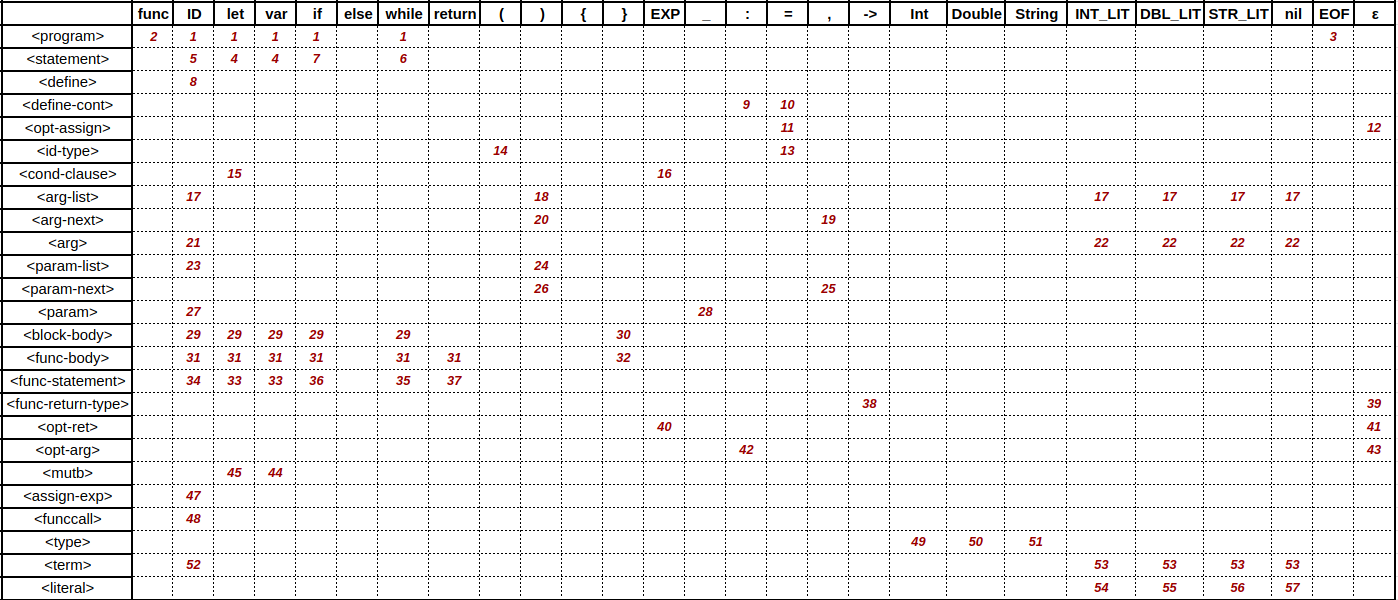
\includegraphics[scale=0.6, angle=-90]{images/ll-table.png}
    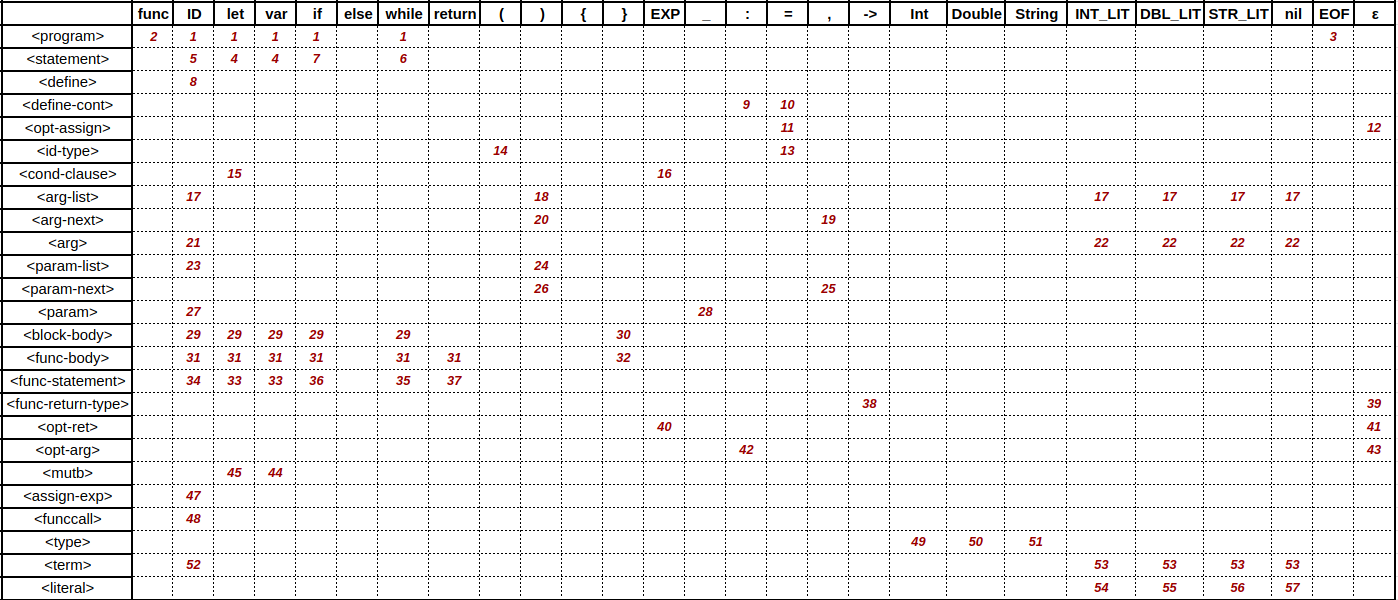
\includegraphics[width=22cm, angle=-90,keepaspectratio]{images/ll-table.png}
\end{center}